%% ----------------------------------------------------------------
%% Thesis.tex -- main
%% ---------------------------------------------------------------- 

\documentclass[a4paper, 10pt, oneside]{memoir}
\usepackage{basilea}

%% ----------------------------------------------------------------

\title				{Thesis Title}
\thesistype			{Thesis Type (e.g., Bachelor/Master thesis/project)}

\department 		    {Department (e.g., Department of Mathematics and Computer Science)}
\faculty			{Faculty (e.g., Natural Science Faculty of the University of Basel)}
\research		    {Research Group \\ Webpage}

\examiner    		{Examiner (e.g., Prof. Dr. Alan Turing)}
\supervisor  		{Supervisor (e.g., Advisor, MSc.)}

\authors     		{Author(s)}
\email				{E-Mail}
\immatriculnr		{0000-000-000}

\date				{Hand-In-Date}

% switch here for the german logo to logo-de
\ulogo				{Template/logo-en} 


%% ----------------------------------------------------------------
\begin{document}

% for english use \selectlanguage{english}, for german use \selectlanguage{ngerman}
\selectlanguage{english}

\thesisfront
\maketitle
\pagestyle{thesis}
%% ----------------------------------------------------------------
% \chapter{Acknowledgments}
%% ----------------------------------------------------------------
\chapter{Abstract}
This thesis discusses the thesis template using some examples of the Turing Machine.
%% ----------------------------------------------------------------
\thesistoc
%% ----------------------------------------------------------------
%\thesisnomencl
%% ----------------------------------------------------------------
\thesismain
\chapter{Introduction}

This is the introduction of the thesis template. The goal\footnote{Furthermore, this document shows how to use the template} is to give students a help to format and style their bachelor's or master's thesis. Please make sure to always use the most current version of this template, by downloading it always from the git repository.\footnote{\url{http://www.github.com/navige/unibas-latex}} By the way, we will use throughout this tutorial some references to Turing's imitation game~\cite{turing:1950} and the Turing machine~\cite{turing:1936}.


% !TEX root = ../Thesis.tex
\chapter{Body of the Thesis}

This is the body of the thesis.

\section{Structure}
\label{sec:my-label}

\subsection{Sub-Section}

\subsubsection{Sub-Sub-Section}

\paragraph{Paragraph}

\subparagraph{Even Sub-Paragraph}

This is the body text. Make sure that when you reference anything you use labels and references. When you refer to anything, you normally capitalise the type of object you reference to, e.g. Section~\ref{sec:my-label} instead of section~\ref{sec:my-label}. You may also just use the \texttt{cref} command and it will generate the label, e.g., for \cref{sec:my-label}, we did not specify the word ``Section''.

Hint: Try to structure your labels as it is done with \texttt{sec:my-label} and \texttt{fig:machine}, etc.



\section{Equations}
A Turing Machine is a 7-Tuple:
\begin{equation}
    M = \langle Q, \Gamma, b, \Sigma, \delta, q_0, F \rangle
\end{equation}
A Turing Machine is a 7-Tuple even if defined in the text, as in $M = \langle Q, \Gamma, b, \Sigma, \delta, q_0, F \rangle$.




\section{Tables}
Some tables can also be used as shown in Table~\ref{tab:table}\footnote{Table captions are normally above the table.}. Remember that tables might be positioned elsewhere in the document. You can force positioning by putting a \texttt{ht!} in the definition.

\begin{table}[ht!]
\centering
\caption{Frequency of Paper Citations. By the way: Make sure to put the label always after the caption, otherwise \LaTeX{} might reference wrongly!}
\begin{tabular}{lcl} \toprule
Title&$f$&Comments\\ \midrule
The chemical basis of morphogenesis & 7327 & \\ 
On computable numbers, with an application to the ... & 6347 & Turing Machine\\
Computing machinery and intelligence & 6130 & \\ \bottomrule
\end{tabular}
\label{tab:table}
\end{table}




\section{Figures}
Figures are nice to show concepts visually. For organising well your thesis, put all figures in the Figures folder. Figure~\ref{fig:machine} shows how to insert an image into your document. Figure~\ref{fig:tm} references a figure with multiple sub-figures. \todoMissing{Description of figure.}

\begin{figure}
\centering
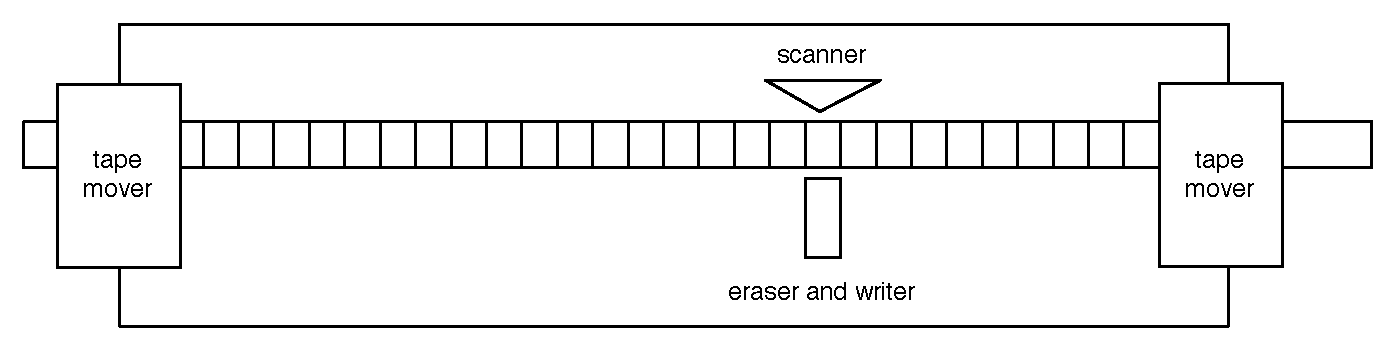
\includegraphics[width=0.9\textwidth]{turingmachine}
\caption{A Turing machine.}
\label{fig:machine}
\end{figure}


\begin{figure}
\centering
\subbottom[Turing Machine 1]{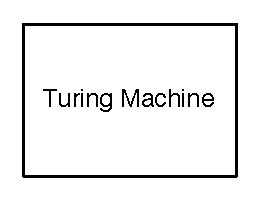
\includegraphics[width=0.2\textwidth]{block}\label{fig:tm:tm1}}
\subbottom[Turing Machine 2]{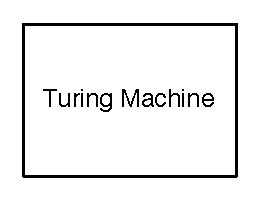
\includegraphics[width=0.2\textwidth]{block}\label{fig:tm:tm2}}
\subbottom[Turing Machine 3]{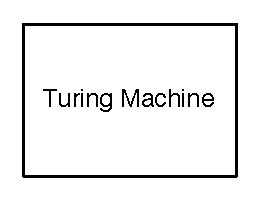
\includegraphics[width=0.2\textwidth]{block}\label{fig:tm:tm3}}
\subbottom[Turing Machine 4]{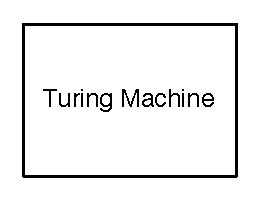
\includegraphics[width=0.2\textwidth]{block}\label{fig:tm:tm4}}
\caption{Plots of four Turing machines}
\label{fig:tm}
\end{figure}




\section{Packages}
These packages might be helpful for writing your thesis:

\begin{description}
	\item[\texttt{caption}] to adjust the look of your captions
	\item[\texttt{glossaries}] for creating glossaries (also list of symbols)
	\item[\texttt{makeidx}] for indexes and the back of your document
	\item[\texttt{algorithm, algorithmicx, algpseudocode}] for adding algorithms to your document
\end{description}
\chapter{Conclusion}
Conclude your thesis with a short conclusion.
%\input{./Chapters/Chapter4}
%\input{./Chapters/Chapter5}
%\input{./Chapters/Chapter6}
%\input{./Chapters/Chapter7}
%% ----------------------------------------------------------------
\thesisappendix
\thesisbib
\begin{appendices}
	\chapter{Appendix} 
\end{appendices}
%% ----------------------------------------------------------------
\thesisback
\chapter[Declaration on Scientific Integrity]{Declaration on Scientific Integrity\\Erklärung zur wissenschaftlichen Redlichkeit}
\label{DeclarationOfAuthorship}

includes Declaration on Plagiarism and Fraud \\
beinhaltet Erklärung zu Plagiat und Betrug \vspace{1cm}

\formlabel{Author}{Autor}
\authorsint

\formlabel{Matriculation number}{Matrikelnummer}
\immatriculnrint

\formlabel{Title of work}{Titel der Arbeit}
\titleint

\formlabel{Type of work}{Typ der Arbeit}
\thesistypeint

\formlabel{Declaration}{Erklärung}
I hereby declare that this submission is my own work and that I have fully acknowledged the assistance received in completing this work and that it contains no material that has not been formally acknowledged. 
I have mentioned all source materials used and have cited these in accordance with recognised scientific rules.

\vspace{0.3cm}

Hiermit erkläre ich, dass mir bei der Abfassung dieser Arbeit nur die darin angegebene 
Hilfe zuteil wurde und dass ich sie nur mit den in der Arbeit angegebenen Hilfsmitteln 
verfasst habe. Ich habe sämtliche verwendeten Quellen erwähnt und gemäss anerkannten wissenschaftlichen Regeln zitiert. 


\vspace*{0.5cm}

Basel, \dateint
\vspace*{0.25cm}

\begin{flushright}
\rule{75mm}{0.4pt} \\
\formlabel{Signature}{Unterschrift}
\end{flushright}

%% ----------------------------------------------------------------
\end{document}
%% ----------------------------------------------------------------
